\documentclass[runningheads]{llncs}

% =====================================================================
% COMPASS -- IJCKG submission (In-Use Track recommended)
% NOTE ON VENUE STYLE: This file keeps the LNCS class so it compiles in
% your existing Overleaf project (llncs.cls + splncs04.bst). If IJCKG
% mandates the ACM sigconf style, switching is mechanical:
%   - replace the \documentclass line and \bibliographystyle,
%   - move \keywords into the ACM \ccsdesc/\keywords block,
%   - the body text below is style-agnostic and can be pasted as-is.
% Confirm the required style on the IJCKG submission page before final.
% =====================================================================

\usepackage[T1]{fontenc}
\usepackage[utf8]{inputenc}

\usepackage{graphicx}
\usepackage{amsmath,amssymb}
\usepackage{booktabs}
\usepackage{enumitem}
\usepackage{placeins}
\usepackage[hidelinks]{hyperref}
\usepackage[strings]{underscore}

% ---- natbib-free compatibility shims ----
\providecommand{\citep}[1]{\cite{#1}}
\providecommand{\citet}[1]{\cite{#1}}

% Helper macro to input auto-generated LaTeX tables that contain underscores
\newcommand{\code}[1]{\texttt{\detokenize{#1}}}
\newcommand{\InputTableSanitized}[1]{%
  \begingroup\catcode`\_=12\relax\input{#1}\endgroup}

% Pretty mode / system names
\newcommand{\Compass}{\textsc{COMPASS}}
\newcommand{\BaseMode}{\textsc{Base}}
\newcommand{\MemMode}{\textsc{Mem}}
\newcommand{\MemSymMode}{\textsc{Mem+Sym}}
\newcommand{\RAGBase}{\textsc{RAG-Base}}
\newcommand{\SymOnly}{\textsc{Sym-Only}}
\newcommand{\RouterMode}{\textsc{Router}}
\newcommand{\RLMode}{\textsc{RL}}
\newcommand{\LongCtx}{\textsc{GPT4o-LongCtx}}
\newcommand{\LogicLM}{\textsc{Logic-LM}}
% Best configuration is COMPASS. The macro below keeps any legacy
% \AdaptiveRAG references compiling and rendering as COMPASS.
\newcommand{\AdaptiveRAG}{\textsc{COMPASS}}

\title{COMPASS: Reliable and Auditable Question Answering\\
for Digital Product Passports}
\titlerunning{COMPASS: Reliable and Auditable QA for Digital Product Passports}
% Double-blind policy: leave author names blank (no dummy names)
\author{}
\institute{}

\begin{document}
\maketitle

\begin{abstract}
Digital Product Passports (DPPs) are emerging as a regulatory and industrial mechanism for exposing product-level technical, compliance, and sustainability information. Question answering over such records is reliability-critical: answers must be grounded in evidence, auditable under scrutiny, and safely withheld when required information is missing or uncertain. Existing retrieval-augmented and long-context LLM systems answer many factual questions but offer limited support for persistent reuse of verified facts, machine-checkable compliance reasoning, and calibrated answer/abstain decisions. We present \Compass, a reliability-first question-answering architecture for DPPs whose foundation is an explicit answer/abstain decision: every output is either an evidence-grounded answer with provenance or a safe abstention. Answers are grounded in three complementary sources---hybrid document retrieval, persistent fact memory, and a targeted symbolic layer that validates compliance-style queries against a CIRPASS-2-aligned DPP ontology within a decidable rule fragment and emits machine-checkable traces. We evaluate \Compass\ in three complementary settings: a 3,429-question DPP reliability suite over partner and public product corpora, a 3,000-question compositional benchmark requiring evidence routing across documents, memory, and structured state, and a 4,021-query out-of-domain study on Open Food Facts. On the reliability suite, \Compass\ improves accuracy from 0.8973 to 0.9749 over a strong retrieval baseline and reduces selective risk (AURC) from 0.5513 to 0.0117; on rule-constrained questions, targeted symbolic validation raises accuracy from 0.0102 to 0.7085 with no observed false positives among rule-fired cases. On the controlled compositional benchmark, \Compass\ answers all cases correctly while strong long-context and Logic-LM baselines fall to 0.68 and 0.64 on the hardest multi-source subtype, and on Open Food Facts it achieves 0.972 accuracy with ECE 0.021 while abstaining on systematically missing fields. These results indicate that targeted symbolic control, provenance-aware evidence composition, and calibrated abstention can make product-record QA more trustworthy and auditable. We release the ontology, rules, dataset-generation scripts, and evaluation harness.
\end{abstract}

\keywords{Digital Product Passports \and reliable question answering \and selective prediction \and auditable AI \and retrieval-augmented generation \and targeted symbolic reasoning \and ontologies \and knowledge graphs \and calibration}

\section{Introduction}
Large Language Models (LLMs) are increasingly deployed to answer questions over technical documentation and semi-structured product records. In regulated product settings, familiar failure modes such as hallucinated properties, unverified compliance claims, and overconfident answers are not merely a usability issue; they can propagate into audits, procurement decisions, sustainability reporting, and downstream supply-chain actions. Digital Product Passports (DPPs) sharpen these requirements by moving product information toward standardized, inspectable, and life-cycle-oriented disclosure, where decisions must remain defensible under external scrutiny \cite{eu2024espr,ec_espr_dpp}. In this context, the central concern is not only whether an answer sounds plausible, but whether it is verifiable, traceable to evidence, and safe to act upon.

This work originates in an applied setting: \Compass\ was developed and exercised within an EU project on circular-economy product information, using real product documentation from industrial partners (a heating-systems manufacturer and a printing-hardware manufacturer) alongside a public battery corpus.\footnote{Project and partner identities are withheld to preserve double-blind review and will be disclosed in the camera-ready version.} The target users are compliance, procurement, and sustainability practitioners outside the development team, for whom an unsupported but confident answer is more costly than an explicit ``don't know.''

Question answering over DPP-like data structures is reliability-critical for three recurring reasons. First, questions often depend on facts introduced far earlier in a product's documentation lifecycle, sometimes across multiple documents and interactions, which makes long-horizon recall essential. Second, many queries are implicitly or explicitly rule-constrained (e.g., obligations, forbidden combinations, ageing constraints), so correctness depends on satisfying structured conditions rather than producing fluent text. Third, the system must be able to abstain when evidence is missing, stale, contradictory, or outside policy. These properties are difficult to guarantee with prompting alone. Even with retrieval, long-context behaviour can be brittle in practice, including sensitivity to where relevant evidence appears within the context window \cite{liu2024lostinthemiddle}, and free-form rationales are not proofs and may be unfaithful to the model's actual decision process \cite{turpin2023unfaithfulcot,lanham2023faithfulnesscot}.

Most current approaches for product-document QA rely on retrieval-augmented generation (RAG) or long-context prompting as the primary mechanism for grounding and factuality. While effective for many factual questions, such systems typically provide limited support for persistent reuse of verified facts across sessions, machine-checkable evidence for compliance-style decisions, and calibrated operating points that explicitly trade off coverage against risk. We therefore take a reliability-first view and treat \emph{answer vs.\ abstain} as a first-class decision, characterizing selective behaviour with risk--coverage curves and AURC and reporting calibration diagnostics (ECE and reliability plots) to support policy-driven operating points \cite{geifman2019selectivenet,kamath2020selectiveqa,guo2017calibration,traub2024aurc}.

The foundation of \Compass\ is a reliability-first answer/abstain decision rather than any single knowledge source. Answers are grounded in three complementary sources: hybrid retrieval and persistent memory handle open-book and long-horizon questions, while a \emph{targeted} symbolic layer validates compliance-style queries against structured facts organized under a DPP ontology, aligned to the CIRPASS-2 EU DPP Core Ontology proposal, and returns machine-checkable rule traces. A post-hoc calibration layer then converts multi-source evidence signals into coverage-targeted answer/abstain decisions. The ontology and rule layer are thus a means to verifiable, auditable validity on the subset of queries where structured constraints apply---not the system's sole knowledge store. Although motivated by DPPs, the architecture is designed to transfer to other structured product records, requiring primarily schema and ontology adaptation rather than redesign of the decision interface.

\noindent Our contributions are:
\begin{itemize}[leftmargin=1.2em,itemsep=2pt,topsep=2pt]
  \item \textbf{A reliability-first QA architecture} (\Compass) for Digital Product Passports that composes hybrid retrieval, persistent fact memory, and a targeted, ontology-backed symbolic layer (aligned to CIRPASS-2) over an explicit, provenance-carrying answer/abstain interface.
  \item \textbf{An evaluation protocol for auditable, selective QA} pairing accuracy with Wilson confidence intervals \cite{wilson1927probable}, selective risk (risk--coverage curves and AURC) \cite{kamath2020selectiveqa,traub2024aurc}, paired significance testing (McNemar) \cite{mcnemar1947note}, calibration diagnostics \cite{guo2017calibration}, and symbolic coverage/precision.
  \item \textbf{Three complementary empirical studies:} a 3,429-question reliability suite on real partner and public corpora; a purpose-built 3,000-question compositional benchmark against strong long-context and neuro-symbolic baselines; and a 4,021-query out-of-domain generalization study on Open Food Facts (drawn from a database of 4.5M products) that stresses calibration and abstention on an unseen schema.
\end{itemize}

\section{Related work}
\paragraph{Retrieval-augmented generation and structured grounding.}
Retrieval-augmented generation (RAG) improves factuality by conditioning the generator on retrieved passages \cite{lewis2020rag}, and hybrid retrieval with fusion-based readers can further improve evidence utilisation \cite{izacard2021fid}. However, retrieval alone does not enforce logical validity or calibrated trust: models may produce fluent but unsupported statements and may fail to use evidence faithfully under long contexts, where positional effects (``lost in the middle'') show that simply increasing context length does not guarantee robust evidence use \cite{liu2024lostinthemiddle}. A separate line of work answers questions \emph{over} a knowledge graph as the primary store (KGQA), enforcing validity through graph structure at the cost of requiring complete graph coverage. \Compass\ occupies a middle ground: it uses retrieval and memory as the primary evidence path for open-book and long-horizon questions, and invokes an ontology-backed symbolic layer only for the compliance-style subset where structured validation adds value---so the ontology supplies targeted validity rather than serving as the sole knowledge source.

\paragraph{Memory-augmented language models.}
External memory mechanisms range from differentiable systems such as Neural Turing Machines and the Differentiable Neural Computer \cite{graves2014ntm,graves2016dnc} to non-parametric retrieval in language modelling \cite{khandelwal2020knnlm}. At scale, retrieval-centric training such as RETRO shows that large external corpora can substitute for parametric capacity in some regimes \cite{borgeaud2022retro}, recurrent memory transformers maintain state beyond a single window \cite{bulatov2022rmt}, and agentic systems emphasise persistent experience stores \cite{wang2023voyager}. Our use of persistent memory is narrower: we store provenance-carrying facts and allow retrieval as a controlled, auditable input to the answerer.

\paragraph{Neuro-symbolic reasoning and verifiability.}
Neuro-symbolic approaches combine learning with explicit inference to improve verifiability and compositional generalisation \cite{riegel2020lnn,dong2019nlm,manhaeve2018deepproblog}. In ontology settings, OWL reasoners such as HermiT provide sound inference over structured knowledge \cite{glimm2014hermit}, and the OWL~2 profiles define fragments (e.g., OWL~2~RL) with favourable computational properties \cite{motik2009owl2profiles}. In the LLM era, systems such as LINC and Logic-LM integrate language models with symbolic inference to improve logical reasoning \cite{olausson2023linc,pan2023logiclm}; we adopt Logic-LM as a baseline. Beyond end-task performance, we contribute deployment-oriented measurements: we quantify where rules apply (symbolic coverage) and how reliable they are when they do (symbolic precision), so that auditability claims are empirically testable rather than rhetorical.

\paragraph{Calibration, selective prediction, and faithful reasoning.}
Neural networks are frequently miscalibrated \cite{guo2017calibration,desai2020calibration}; selective prediction formalises abstention and studies risk under coverage constraints \cite{kamath2020selectiveqa,geifman2019selectivenet}, and AURC provides a compact summary of risk--coverage behaviour \cite{traub2024aurc}. Reasoning-through-language can be effective yet unfaithful \cite{turpin2023unfaithfulcot,lanham2023faithfulnesscot}, and tool-using prompting such as ReAct improves factuality without formal guarantees or calibration \cite{yao2022react}. \Compass\ reduces unfaithfulness by constraining the answerer to retrieved evidence and explicit symbolic traces, and measures abstention via selective-risk analysis.

\section{Problem formulation and metrics}
Given a query $x$ about a specific product and its documentation, the system outputs either (i) an answer $y$ with provenance (citations and/or a rule trace) or (ii) an abstention symbol $\bot$. The system operates over a domain corpus (technical documents) and a structured knowledge layer (ontology + facts), and targets reliability-critical workflows where ``don't know'' is safer than a confident but unsupported answer. A confidence score $c(x)\in[0,1]$ and a threshold $\tau$ define a selective predictor,
\[
\hat{y}(x)=
\begin{cases}
  y(x), & c(x) \ge \tau \\
  \bot, & c(x) < \tau,
\end{cases}
\]
where \emph{coverage} is the fraction of instances answered and \emph{risk} is the error rate among answered instances. We summarise the risk--coverage trade-off with AURC (lower values indicate that errors concentrate at low confidence and can be avoided by abstention) \cite{kamath2020selectiveqa,traub2024aurc}. Because operating points are policy choices---mandated minimum coverage in customer support versus stricter abstention in compliance auditing---we report the entire curve rather than a single threshold.

Calibration is reported as expected calibration error (ECE), the weighted average gap between per-bin confidence and per-bin accuracy \cite{guo2017calibration,desai2020calibration}. Because calibration is not arithmetically implied by high accuracy, we treat it as a separate reliability axis. To avoid over-interpreting small differences we report Wilson score 95\% confidence intervals \cite{wilson1927probable}, which are well-behaved near 0 and 1, and McNemar's exact test for paired comparisons on identical question sets \cite{mcnemar1947note}. Finally, we report symbolic \emph{coverage} (fraction of questions triggering at least one rule) and symbolic \emph{precision} (correctness conditional on firing), isolating where explicit rules contribute and where the system relies on retrieval or memory.

\section{The COMPASS architecture}
\subsection{Overview}
Figure~\ref{fig:architecture} summarizes the end-to-end inference path. A query triggers hybrid evidence acquisition from the document corpus and the persistent memory store; for compliance-style queries, structured facts are checked by an ontology-backed symbolic layer that emits both conclusions and auditable traces; a context-bound LLM answerer composes only from sanctioned evidence; and a post-hoc calibration layer maps raw confidence to a calibrated score, with a threshold $\tau$ deciding between an answer with provenance and a safe abstention.

\begin{figure}[t]
\centering
\makebox[\linewidth][c]{%
    \includegraphics[width=1.05\linewidth,height=0.45\textheight]{architecture_overview-2.png}
}
\caption{Overview of the \Compass\ architecture. Hybrid evidence acquisition draws on the document corpus and persistent memory; structured facts are checked by the ontology-backed knowledge-graph layer, which emits conclusions and machine-checkable rule traces; a context-bound answerer composes only from sanctioned evidence; and post-hoc calibration with threshold $\tau$ yields an answer with citations and rule traces or an abstention.}
\label{fig:architecture}
\end{figure}

\subsection{Evidence acquisition: hybrid retrieval and persistent memory}
We use a hybrid retriever combining sparse lexical and dense embedding retrieval (with optional reranking), consistent with evidence that hybrids often outperform purely dense or sparse retrieval on heterogeneous corpora \cite{lewis2020rag,izacard2021fid}; the retriever returns passages with provenance identifiers. Persistent memory stores validated facts with provenance (e.g., extracted component types, test reports, dates). At query time, memory facts are retrieved by semantic similarity and merged with the retrieval context, supporting long-horizon recall beyond a single prompt and mitigating long-context brittleness. A recurring failure mode in document-grounded QA is that the generator mixes retrieved evidence with unsupported extrapolation; to mitigate this, the answerer is constrained to a \emph{context pack}: a deduplicated set of evidence snippets and memory facts, each annotated with a provenance identifier that is surfaced as a citation and logged for audit.

\subsection{Targeted symbolic validation over a DPP ontology}
Validated product facts are represented as RDF triples under a DPP ontology aligned to the CIRPASS-2 EU DPP Core Ontology proposal \cite{cirpass2}: core classes (Product, Component, Material, Process\-Step, Standard) carry \texttt{skos:closeMatch}/\texttt{exactMatch} links to the corresponding CIRPASS-2 terms, and object properties (\texttt{hasComponent}, \texttt{usesMaterial}, \texttt{requiresCompliance}, \texttt{requiresStep}, \texttt{conformsTo}) connect them. Per-domain ontologies (battery, printing hardware, heating systems, and---for the generalization study---textiles and food) specialise this core with domain classes and standards.

To keep reasoning sound and terminating, the schema is restricted to a decidable fragment: class and property assertions, subclass and subproperty axioms, and domain/range restrictions, evaluated within OWL~2~RL semantics \cite{motik2009owl2profiles} and complemented by forward-chaining compliance rules. This design choice matters for deployment: it guarantees the rule evaluator terminates regardless of input, rather than relying on full OWL-DL classification. Obligation rules have the form
\[
\texttt{hasComponent}(p,c) \wedge \texttt{type}(c,t) \Rightarrow \texttt{requiresCompliance}(c,s),
\]
where $p$ is a product, $c$ a component, $t$ a component class, and $s$ a standard; constraint rules act as conservative vetoes (missing required fields, stale reports, out-of-window dates). When rules contribute, the system returns a machine-checkable trace---which rule fired and which triples matched---so that reviewers and auditors can distinguish rule-derived conclusions from purely neural generations. Sound inference over the ontology is provided by HermiT-style reasoning \cite{glimm2014hermit}. Consistent with our measurements (Section~\ref{sec:reliability}), the symbolic layer is deliberately \emph{targeted}: it fires only where structured facts and a matching rule exist, providing high-precision control over the compliance-style subset rather than broad coverage of all questions.

\subsection{Calibration, confidence, and modes}
Selective prediction requires a scalar confidence score. Rather than assuming the LLM's raw generation probability is well-calibrated, \Compass\ aggregates signals from retrieval-score margins, agreement across evidence snippets, symbolic fire flags, and (when available) generation probabilities into an uncalibrated score $\hat{c}(x)$, then fits a monotone post-hoc calibrator $g$ on development data to produce $c(x)=g(\hat{c}(x))$; isotonic regression is a standard choice \cite{zadrozny2002transforming,guo2017calibration}. At deployment, $\tau$ is selected to meet policy-driven coverage constraints on a held-out split and then applied unchanged to test data.

The evaluation harness exports several \emph{modes} that we treat as ablations of the full design: \RAGBase\ (retrieval-only), \MemMode\ (adds memory), \SymOnly\ (symbolic-only), \MemSymMode\ (memory+symbolic), \RouterMode\ (supervised router), and \Compass\ (the full configuration). A reinforcement-learned router (\RLMode) is reported only for completeness in the reliability suite and is not claimed as a contribution, since its paired tests do not show significant improvement.

\section{Experimental setting}
\subsection{Studies and data}
We report three complementary studies. (1) A \emph{reliability suite} of 3,429 DPP-aligned questions over three corpora---a battery corpus and two manufacturer-specific product-documentation corpora---categorised as \textbf{logic} (rule-constrained compliance), \textbf{open} (open-book extraction), and \textbf{recall} (long-horizon persistence); counts appear in Table~\ref{tab:counts}. (2) A purpose-built \emph{compositional architecture benchmark} of 3,000 questions whose subtypes require routing across document evidence, persistent memory, and structured system state (e.g., \texttt{memory+document}, \texttt{memory+document+symbolic}); this benchmark targets exactly the multi-source cases that single-mechanism systems handle poorly. (3) An \emph{out-of-domain generalization} study on Open Food Facts (OFF), a public database of 4.5M food products with 210 fields, from which we generated context-bound evaluation queries spanning nutrition, attribute, missingness, sustainability, and fairness types.

\begin{table}[t]
\centering
\small
\InputTableSanitized{docs/paper/tables/dataset_counts.tex}
\caption{Reliability-suite question counts by corpus and query type (pooled total $n{=}3429$).}
\label{tab:counts}
\end{table}

\subsection{Baselines}
In the reliability suite we compare against \RAGBase\ (a strong hybrid-retrieval baseline) and the ablation modes above. In the compositional benchmark we additionally compare against two strong external baselines: \LongCtx, a long-context LLM given all relevant evidence in-context \cite{liu2024lostinthemiddle}, and \LogicLM, an LLM coupled to a symbolic solver \cite{pan2023logiclm}. All quantitative results are produced by an automated pipeline and exported directly into paper-ready tables and figures to reduce transcription error and support reproducibility.

\section{Results}
\label{sec:reliability}
\subsection{Reliability suite: pooled performance}
Table~\ref{tab:summary} reports pooled test-set performance. The final three columns summarize average pathway usage within the shared harness (fraction of queries invoking retrieval, fraction triggering symbolic checks, and a proxy latency index); these characterize relative pathway cost within the harness and are not deployment latency benchmarks. For \RLMode, the ``Retrieval use'' and ``Symbolic checks'' entries are not directly comparable, because the policy is evaluated as an end-to-end controller whose internally composed actions are not decomposed into per-module counters; the printed zeros should be read as ``not separately attributed.'' The strongest overall mode is \Compass: pooled accuracy 0.9749 (CI 0.9691--0.9796) and AURC 0.0117, whereas \RAGBase\ reaches 0.8973 (CI 0.8867--0.9071) with substantially worse selective risk (AURC 0.5513).

\begin{table}[t]
\centering
\footnotesize
\setlength{\tabcolsep}{4pt}
\renewcommand{\arraystretch}{1.05}
\begin{tabular}{lcccccc}
\toprule
Method & Acc. & 95\% CI & AURC & Retrieval & Symbolic & Proxy latency \\
 &  &  &  & use & checks & (ms) \\
\midrule
\Compass & 0.9749 & [0.9691, 0.9796] & 0.0117 & 0.934 & 0.080 & 7560 \\
\RAGBase & 0.8973 & [0.8867, 0.9071] & 0.5513 & 1.000 & 0.000 & 8281 \\
\RLMode & 0.8965 & [0.8858, 0.9062] & 0.4227 & 0.000 & 0.000 & 17 \\
\MemSymMode & 0.5777 & [0.5611, 0.5942] & 0.1387 & 0.312 & 0.080 & 9 \\
\MemMode & 0.5001 & [0.4834, 0.5169] & 0.3469 & 0.312 & 0.000 & 380 \\
\SymOnly & 0.0965 & [0.0871, 0.1069] & 0.4556 & 0.000 & 0.080 & 3 \\
\RouterMode & 0.0869 & [0.0779, 0.0968] & 0.4667 & 0.000 & 0.080 & 723 \\
\BaseMode & 0.0169 & [0.0131, 0.0218] & 0.9915 & 0.000 & 0.000 & 1 \\
\bottomrule
\end{tabular}
\caption{Pooled results on the 3,429-question reliability suite. ``Retrieval use'' and ``Symbolic checks'' denote the average fraction of queries invoking retrieval and rule evaluation; ``Proxy latency'' is an exporter-side pathway-cost proxy, not an end-to-end serving benchmark.}
\label{tab:summary}
\end{table}

The paired McNemar comparison (Table~\ref{tab:mcnemar}) confirms the gain is not an artifact of small differences: \Compass\ corrects 266 instances that \RAGBase\ answers incorrectly, with none in the reverse direction ($p<10^{-6}$).

\begin{table}[t]
\centering
\small
\setlength{\tabcolsep}{5pt}
\renewcommand{\arraystretch}{1.05}
\begin{tabular}{lcccr}
\toprule
Method A & Method B & A-only wins & B-only wins & Exact $p$ \\
\midrule
\Compass & \RAGBase & 266 & 0 & $<10^{-6}$ \\
\bottomrule
\end{tabular}
\caption{Exact paired McNemar comparison on the pooled reliability suite. ``A-only wins'' denotes instances answered correctly by A and incorrectly by B.}
\label{tab:mcnemar}
\end{table}

\subsection{Reliability suite: where the gains come from}
Table~\ref{tab:types} shows a sharp task-type separation. Open questions are near ceiling because many are short extractive queries whose answer span appears verbatim in the retrieved evidence; we therefore read exact 1.000 values as benchmark saturation on this snapshot, not as a claim that open-book QA is solved. The discriminative setting is \textbf{logic}: \Compass\ lifts rule-constrained accuracy from 0.0102 (\RAGBase) to 0.7085, and \SymOnly\ reaches 0.9051, directly demonstrating the value of explicit symbolic support. \Compass\ is thus best understood as preserving the strong open and recall behaviour of retrieval-centric modes while substantially improving logic performance.

\begin{table}[t]
\centering
\small
\setlength{\tabcolsep}{5pt}
\renewcommand{\arraystretch}{1.05}
\begin{tabular}{lccc}
\toprule
Method & Logic & Open & Recall \\
\midrule
\Compass & 0.7085 & 1.0000 & 1.0000 \\
\RAGBase & 0.0102 & 1.0000 & 0.9283 \\
\RLMode & 0.0034 & 1.0000 & 0.9271 \\
\MemSymMode & 0.7085 & 0.5320 & 0.6571 \\
\MemMode & 0.0136 & 0.5320 & 0.5842 \\
\SymOnly & 0.9051 & 0.0000 & 0.0765 \\
\RouterMode & 0.7932 & 0.0000 & 0.0765 \\
\BaseMode & 0.1966 & 0.0000 & 0.0000 \\
\bottomrule
\end{tabular}
\caption{Accuracy by query type on the pooled reliability suite. Exact 1.000 values reflect extractive saturation on this frozen snapshot.}
\label{tab:types}
\end{table}

The risk--coverage curves (Figure~\ref{fig:riskcov}) show \Compass\ dominating \RAGBase\ across operating points, consistent with the AURC reductions in Table~\ref{tab:summary}. Table~\ref{tab:symcov} quantifies the symbolic layer honestly: it fires on 273 of 3,429 questions (7.96\%) with no observed false positives. We therefore frame the symbolic component as \emph{targeted, high-precision control} over the compliance subset rather than a broad-coverage mechanism, and attribute the system's overall reliability to the combination of this targeted control with calibrated, evidence-grounded abstention.

\begin{figure}[t]
\centering
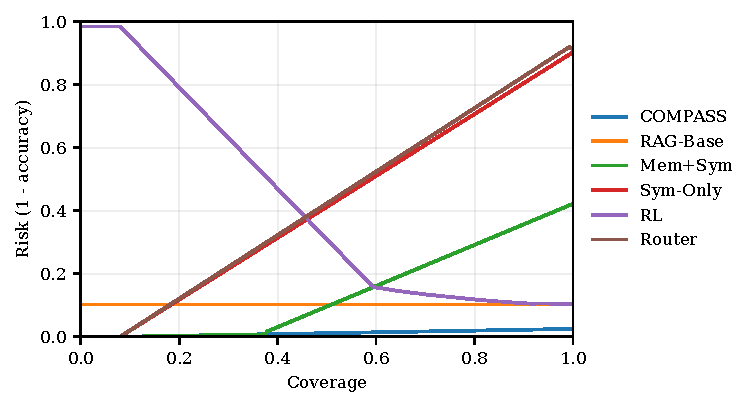
\includegraphics[width=0.9\linewidth]{artifacts/risk_coverage.png}
\caption{Risk--coverage curves on the reliability suite. Lower risk at the same coverage indicates safer selective behaviour.}
\label{fig:riskcov}
\end{figure}

\begin{table}[t]
\centering
\small
\setlength{\tabcolsep}{5pt}
\renewcommand{\arraystretch}{1.05}
\begin{tabular}{lcccc}
\toprule
Method & Questions & Rule-fired & Coverage & Precision when fired \\
\midrule
\Compass & 3429 & 273 & 0.0796 & 1.000 \\
\MemSymMode & 3429 & 273 & 0.0796 & 1.000 \\
\SymOnly & 3429 & 273 & 0.0796 & 1.000 \\
\RouterMode & 3429 & 273 & 0.0796 & 1.000 \\
\RAGBase & 3429 & 0 & 0.0000 & --- \\
\bottomrule
\end{tabular}
\caption{Symbolic coverage and conditional precision on the reliability suite (modes with zero rule firings omitted for space).}
\label{tab:symcov}
\end{table}

\subsection{Compositional architecture benchmark}
The reliability suite saturates on open and recall questions, limiting its power to separate architectures. We therefore evaluate on a purpose-built 3,000-question benchmark whose subtypes require composing evidence across documents, memory, and structured state. Table~\ref{tab:arch} reports the result. \Compass\ is correct on all 3,000 questions, including every multi-source subtype, whereas the strong baselines degrade precisely where composition is required: \LongCtx\ drops to 0.684 and \LogicLM\ to 0.640 on \texttt{memory+document+symbolic}. Both baselines remain near-perfect on single-mechanism subtypes, confirming that the gap is specific to multi-source composition rather than to any single capability.

\begin{table}[t]
\centering
\small
\setlength{\tabcolsep}{6pt}
\renewcommand{\arraystretch}{1.05}
\begin{tabular}{lccc}
\toprule
Subtype & \Compass & \LongCtx & \LogicLM \\
\midrule
Overall (3000) & \textbf{1.000} & 0.958 & 0.940 \\
\midrule
atomic\_verified (1500) & 1.000 & 0.985 & 0.971 \\
memory+document (225) & 1.000 & 0.871 & 0.751 \\
memory+document+symbolic (225) & \textbf{1.000} & \textbf{0.684} & \textbf{0.640} \\
memory+symbolic compliance (375) & 1.000 & 1.000 & 1.000 \\
memory+symbolic component (375) & 1.000 & 0.989 & 1.000 \\
memory+symbolic step (300) & 1.000 & 1.000 & 1.000 \\
\bottomrule
\end{tabular}
\caption{Accuracy on the 3,000-question compositional benchmark. The gap concentrates on multi-source subtypes (bold), where baselines must combine document, memory, and symbolic evidence.}
\label{tab:arch}
\end{table}

\subsection{Out-of-domain generalization: Open Food Facts}
To test transfer to an unseen schema, we apply the same architecture to Open Food Facts. Real OFF data is highly incomplete (e.g., environmental-score grade present for only $16.6\%$ of products, Nutri-Score for $30.4\%$), making principled abstention essential. Table~\ref{tab:off} reports the row-context evaluation over 4,021 queries. The system attains 0.972 overall accuracy with well-calibrated confidence (ECE 0.021) and low selective risk (AURC 0.025), abstaining heavily on sustainability and nutrition queries where the required fields are systematically missing while answering attribute and missingness queries at high accuracy. Notably, calibration here is far better than the strongest in-domain configuration (Section~\ref{sec:disc}), indicating that the calibration pipeline is effective when confidence signals are well-aligned with evidence availability.

\begin{table}[t]
\centering
\small
\setlength{\tabcolsep}{6pt}
\renewcommand{\arraystretch}{1.05}
\begin{tabular}{lcccccc}
\toprule
Query type & $n$ & Accuracy & Abstain & Coverage & ECE & AURC \\
\midrule
All & 4021 & 0.972 & 0.270 & 0.730 & 0.021 & 0.025 \\
\midrule
nutrition & 1450 & 1.000 & 0.304 & 0.696 & 0.004 & 0.000 \\
attribute & 1146 & 0.998 & 0.002 & 0.998 & 0.002 & 0.000 \\
missingness & 367 & 0.929 & 0.000 & 1.000 & 0.071 & 0.084 \\
sustainability & 1039 & 0.919 & 0.620 & 0.380 & 0.060 & 0.071 \\
fairness & 19 & 1.000 & 0.000 & 1.000 & 0.000 & 0.000 \\
\bottomrule
\end{tabular}
\caption{Out-of-domain results on Open Food Facts (row-context evaluation, $n{=}4021$). Accuracy counts correct abstentions. The system abstains where required fields are systematically missing (sustainability, nutrition) and answers confidently where evidence is present (attribute, missingness).}
\label{tab:off}
\end{table}

\section{Discussion and limitations}
\label{sec:disc}
\paragraph{What drives reliability.}
The most discriminative signals for DPP reliability are logic accuracy, the compositional benchmark, and the selective-risk curves---not pooled open accuracy, which saturates because retrieved evidence often contains the answer verbatim. Our results support a precise claim: reliability comes from the \emph{combination} of targeted, high-precision symbolic control (perfect precision on the 7.96\% rule-fired subset; large gains on logic and multi-source composition) and calibrated, evidence-grounded abstention (low AURC, strong out-of-domain calibration). We do not claim that broad symbolic coverage or calibrated confidence alone explains the gains.

\paragraph{Calibration.}
In-domain ECE can remain high even for the strongest accuracy configuration, motivating conservative operating points and further uncertainty estimation. The Open Food Facts study shows the calibration pipeline performs well (ECE 0.021) when confidence signals align with evidence availability, so we treat calibration as a measured reliability axis that is domain-sensitive rather than a uniformly solved property.

\paragraph{Scope.}
The reliability suite covers three DPP corpora; the compositional benchmark and the Open Food Facts study extend the evaluation to multi-source reasoning and to an unseen schema, respectively. Generalisation to further product categories, normative documents, and shifting regulatory constraints remains future work, and compliance-critical decisions should retain human oversight.

\section{Reproducibility and ethics}
\paragraph{Reproducibility.}
Evaluation outputs are generated by an automated harness and exported directly into the tables and figures above. We release an anonymised repository containing the ontology and rule set, the evaluation harness, the dataset construction scripts for the compositional benchmark, and version identifiers/checksums for data and model checkpoints; the link is provided at submission and de-anonymised after acceptance.

\paragraph{Ethics and responsible use.}
This work targets factual, document-grounded product information and explicitly supports abstention when evidence is missing. The system can still fail under distribution shift (new product categories, altered documentation practices, changed regulations) and should be used with human oversight for compliance-critical decisions. We recommend that deployments expose provenance by default (citations / rule traces) and log abstentions and overrides to enable auditing.

\section{Conclusion}
We presented \Compass, a reliability-first QA architecture for Digital Product Passports that composes hybrid retrieval, persistent memory, and a targeted, ontology-backed symbolic layer (aligned to CIRPASS-2) over an auditable answer/abstain interface. Across three complementary studies (3,429, 3,000, and 4,021 questions), \Compass\ substantially improves selective risk and rule-constrained accuracy over a strong retrieval baseline, answers all cases of a controlled compositional benchmark where strong long-context and neuro-symbolic baselines degrade on multi-source reasoning, and transfers to an unseen Open Food Facts schema with well-calibrated, abstention-aware behaviour. The results show that pairing targeted symbolic control with calibrated abstention yields trustworthy, auditable QA for structured product documentation, while in-domain probability calibration remains a measurable open challenge.

\paragraph{Generative AI use disclosure.}
During manuscript preparation, generative AI tools were used only for minor language support (spelling, grammar, and limited phrasing refinement). They were not used for the research contribution, experimental design, result generation, interpretation, or conclusions. The authors reviewed and approved the final manuscript and take full responsibility for its content.

\bibliographystyle{splncs04}
\bibliography{refs}

\end{document}
